%
%   This file is part of the APS files in the REVTeX 4 distribution.
%   Version 4.0 of REVTeX, August 2001
%
%   Copyright (c) 2001 The American Physical Society.
%
%   See the REVTeX 4 README file for restrictions and more information.
%
% TeX'ing this file requires that you have AMS-LaTeX 2.0 installed
% as well as the rest of the prerequisites for REVTeX 4.0
%
% See the REVTeX 4 README file
% It also requires running BibTeX. The commands are as follows:
%
%  1)  latex apssamp.tex
%  2)  bibtex apssamp
%  3)  latex apssamp.tex
%  4)  latex apssamp.tex
%
%\documentclass[prb,aps,nobibnotes,twocolumn,doublespace,twocolumngrid,superbib]{revtex4}
\documentclass[twocolumn,showpacs,preprintnumbers,amsmath,amssymb]{revtex4}
%\documentclass[preprint,showpacs,preprintnumbers,amsmath,amssymb]{revtex4}

% Some other (several out of many) possibilities
%\documentclass[preprint,aps]{revtex4}
%\documentclass[preprint,aps,draft]{revtex4}
%\documentclass[prb]{revtex4}% Physical Review B

\usepackage{graphicx}% Include figure files
\usepackage{dcolumn}% Align table columns on decimal point
\usepackage{bm}% bold math

%\nofiles

\begin{document}

%\preprint{APS/123-QED}

\title{The linear scaling self-consistent perturbed projection method for high order response}
%\title{\emph{Ab-inito} hyperpolarizabilities by O(N) perturbed projection}% Force line breaks with \\

\author{Val\'ery Weber}
% \altaffiliation[Also at ]{Physics Department, XYZ University.}%Lines break automatically or can be forced with \\
 \email{vweber@t12.lanl.gov}
\author{Anders M. N. Niklasson}%
\author{Matt Challacombe}%

\affiliation{
Los Alamos National Laboratory, Theoretical Division, Los Alamos 87545, New Mexico, USA.\\
}%

\date{\today}% It is always \today, today,
             %  but any date may be explicitly specified

\begin{abstract}
A first principles linear scaling electronic structure scheme for high order 
response properties is proposed. The sheme solves the coupled perturbed self 
consistent field equation by the perturbed projection method. It is applied to 
the computation of the first and second electric hyperpolarizabilities of three
dimensional water clusters. Linear scaling and locality of the response
densities are demonstrated. 
% Linear scaling self consisitent sheme for high order response peoperties
% is proposed. The sheme solves the coupled perturbed self consitent field 
% equation by the perturbed projection method. It is applied to the computation
% of the first and second electric hyperpolarizabilities of three
% dimensional water clusters. Linear scaling and locality of the response
% densities are demonstrated. 
\end{abstract}

%\pacs{Valid PACS appear here}% PACS, the Physics and Astronomy
                             % Classification Scheme.
%\keywords{Suggested keywords}%Use showkeys class option if keyword
                              %display desired
\maketitle


\section{Introduction}
 Electronic structure theory based on the first principle 
 of physics was for long time limitied to the study of small 
 systems with only a small number of nonequivalent atoms. 
 Despite a tremendous increase in computational power
 of digital computers this would still be a severe limitation
 if not more efficient theoretical and computational
 tools were developed. During the last 10 years a new paradigm 
 has evolved in electronic structure theory, where
 no single part of a calculation is allowed to increase in 
 computational complexity more than linearly with the number
 of atoms. 

 Algorithms in linear scaling self-consistent-field (SCF) theory 
 exploit the quantum locality (or nearsightedness) of non-metallic systems, 
 manifested in the approximate exponential decay of the density matrix 
 with atom-atom separation, through the effective use of sparse 
 matrix methods. For small systems this is usually an inefficient
 approach, but for large systems consisting of millions
 of atoms it will have a major future impact, bridging the gap
 between material science, chemistry and biology. So far, most 
 attentions in linear scaling electronic structure
 theory has been focused on total energy calculations and little
 attention has been devoted to the problem of materials response
 properties, such as magnetic and electric responses or nuclear
 displacement. However, the locality principle is extandable
 also to response properties. In previous studies linear scaling 
 for the calculation of response propertie was demonstrated for one
 dimensional linear chain systems (CHECK IT)
 \cite{Ochsenfeld_1997,Ochsenfeld_1998,chintoc}. Recently
 a perturbed projection algorithm was proposed for low order
 response properties for which linear scaling was demonstrated
 also for three dimensional systems \cite{Weber_Niklasson_Challacombe_2004}.

 In the calculation of materials response properties within 
 Hartree-Fock or density functional theory the electronic
 response is given from self-consistent solutions of both
 the ground state density and its perturbative response functions,
 refered to as the solutions to the coupled perturbed self consistent 
 field (CPSCF) equations.
 Standard non-linear scaling approaches to solutions of the CPSCF equations 
 \cite{Pople_1979,Sekino_1986,Dupuis_1991} do not admit full exploitation 
 of locality and sparse matrix algebra, as they are based on perturbation 
 of the wave functions, requiring a solution of the eigenvalue problem
 that scales as ${\cal O}(N^3)$ and with transformation of two-electron
 integrals that typically scales as ${\cal O}(N^5)$ with system size.
 These problems are avoided in a density matrix approach, where both
 the density matrix and its derivatives are calculated directly.
 A few linear scaling response schemes have been proposed.
 Ochsenfeld and Head-Gordon developed a scheme based on the
 Li-Nunes-Vanderbilt density matrix functional \cite{Ochsenfeld_1997}
 and later Larsen {\em et al.} \cite{Helgaker_2001} proposed iterative 
 solutions to the CPSCF equations based on unitary operations
 invovling matrix exponentials. In both of these approaches, a linear 
 system of equations containing commutation relations must be solved.
 Another very interesting approach was demonstrated by Chintoc, who
 derived the frequency response of one dimensional molecular chains
 by calculating the time evolution of the density matrix from
 the quantum-Liouville equation.

 Our approach to linear scaling response theory is quite different 
 from previous attempts. It is based on the perturbed projection
 method in density matrix perturbation theory, recently developed
 by the authors \cite{Niklasson04,Weber04}. With this theory it
 was possible to demonstrate efficient linear scaling {\em ab initio}
 computations for the first electric polarizability of three-dimensional 
 water clusters.

 In this article, we present a linear scaling self consisitent sheme
 for higher order response peoperties up fourth order in energy.
 First we give a general description through the solution of the CPSCF equations.
 Then we describe the perturbed projection approach for the calculation
 of the density matrix derivatives and present
 an algorithm for derivatives up to third order.
 Thereafter, we derive a density matrix analogy to Wigner's 2n+1
 rule for nonorthogonal representations. We also briefly discuss the
 self concistent accelaration technique by Weber and ... . In the next section,
 we first show the saturation of the hyperpolarizabilities up to fourth order
 for a series of 1D chain of water molecules. Thereafter, we demonstate
 linear scaling computation of the higher order electric response properties
 for 3D water clusters.



\section{CPSCF equations}
The coupled perturbed self concistent field equations occur in Hartree-Fock
and density functional theory for the computation of material response
properties. Here, we discuss the CPSCF equation in the framework of
HF theory, however an extension to DFT is straightforward.


The following schematic algorithm is a higher order generalization of the
SC scheme for the solution of the CPSCF equations descibe in \cite{SV} 
based on perturbed pronjection:
\begin{subequations}
\begin{eqnarray}
&&  F^{ab\ldots}_{n}=\mu_a+J(D^{ab\ldots}_n)+K(D^{ab\ldots}_n) \label{FockBuild} \\
&& \displaystyle\widetilde{F}^{ab\ldots}_{n}=\sum_{k=n-m}^{n}c_k F^{ab\ldots}_{k} \label{DDIIS} \\
&& \displaystyle\mathcal{D}^{ab\ldots}_{n+1}=
  \frac{\partial^N}{\partial\mathcal{E}^a \partial\mathcal{E}^b\ldots}
     \theta(\tilde{\mu}I-(\mathcal{F}^{0}
     +\mathcal{E}^{a}\widetilde{\mathcal{F}}^{a}_n
     +\mathcal{E}^{b}\widetilde{\mathcal{F}}^{b}_n+\ldots))
     \bigg|_{\mathcal{E}=0} \label{DDeriv}
   \end{eqnarray} 
\end{subequations}

The scheme solves for the self concistent density response, \\
first... Linear scaling construction of the Fockian expansion follows in
the same way as the O(N) construction of the Fockian cite{Matt...}\\
second... DDIIS optimizing scheme based on DIIS.\\
third... density matrix derivative through perturbation projection.\\


%with starting point $D^a_0=0$. In step~(\ref{FockBuild}),  $F^a_n$ is constructed in 
%${\cal O}(N)$ using algorithms \cite{MChallacombe97,ESchwegler97} in 
%the {\sc MondoSCF} \cite{MondoSCF} suite of linear scaling quantum chemistry programs.
\subsection{DDIIS}

\subsection{Perturbed projection}
Perturbed projection is based on purification projections for the 
construction of the density matrix...

\begin{equation}
  D^{ab\ldots}=D^{ba\ldots}=\ldots
\end{equation}


\begin{subequations}
  \begin{eqnarray}
    && D^{abc}=\{D^{abc},D_0\}+
        \frac{1}{3}(\{D^{ab},D^{c}\}+\{D^{ac},D^{b}\}+\{D^{bc},D^{a}\})\\
    && D^{ab }=\{D^{ab},D_0\}+\frac{1}{2}\{D^{a},D^{b}\}\\
    && D^{a  }=\{D^{a},D_0\}
  \end{eqnarray}
\end{subequations}


\begin{equation}\label{PP1}
  \left.
  \begin{array}{ll}
    X^{ab}_{i+1}&=\{X^{ab}_{i},X^0_{i}\}+\frac{1}{2}\{X^a_{i},X^b_{i}\}\\
    X^a_{i+1}&=\{X^a_{i},X^0_{i}\}\\
    X^b_{i+1}&=\{X^b_{i},X^0_{i}\}\\
    X^0_{i+1}&=(X^0_{i})^2
  \end{array} 
  \right\}\quad {\rm Tr}[X^0_{i}]\ge N_e 
\end{equation}
or 
\begin{equation}\label{PP2}
  \left.
  \begin{array}{ll}
    X^a_{i+1}&=2 X^a_{i}-{X^a_{i},X^0_{i}} \\
    X^0_{i+1}&=2 X^0_{i}-(X^0_{i})^2
  \end{array} 
  \right\}\quad {\rm Tr}[X^0_{i}]< N_e.
\end{equation}



\subsubsection{Algorithm}
...\\
\begin{figure}[htbp]
  \centering
  \caption{\protect
    ..............
  }\label{fig:algo}
\begin{verbatim}
 h = sort(eig(F))
 X = (h(N)*I-F)/(h(N)-h(1))
 D1 = -dF/(h(N)-h(1))
 D2 = 0
 D3 = 0
 Error = 1
 while Error > eps
   if trace(X) > Ne
     D3 = X*D3+D3*X+D1*D2+D2*D1
     D2 = X*D2+D2*X+D1*D1
     D1 = X*D1+D1*X
     X = X*X
   else
     D3 = 2*D3-(X*D3+D3*X+D1*D2+D2*D1)
     D2 = 2*D2-(X*D2+D2*X+D1*D1)
     D1 = 2*D1-(X*D1+D1*X)
     X = 2*X-X*X
   end
   Error = abs(trace(X)-Ne)+abs(trace(D3))
 end
 E0 = trace( X*F)
 E1 = trace( X*dF)/1
 E2 = trace(D1*dF)/2
 E3 = trace(D2*dF)/3
 E4 = trace(D3*dF)/4
\end{verbatim}
\end{figure}


\subsubsection{Higher order response and Wigner's 2n+1 rule }
Higher order energy derivatives can be calculated from the lower
order response. Wigner's 2n+1 rule gives a general way to calculate the 2n+1
energy response from the n-th order response. A density matrix analogy to
the Wigner's 2n+1 rule was given in cite{...}, here we will present
a generalization to the non orthogonal case for mixte derivatives 
up to fourth order....
\section{Examples}
To demonstrate the ability, accuracy and numerical stability we present
...
\subsection{One dimensional water chains}
figures ... show the saturation ....
table shows comparison to 2n+1 and n+1.
10-th order (at least +2n+1 til 21-th order in E (for Anders)).
\subsection{Linear scaling: 3D water clusters}
3D water clusters show an early onset of linear scaling for accrurate
basis set and low tresholds and higher order response.

The density responses matrices show an exponential decay as a function
of the internuclear distance, however the decay is slower and the locality
becomes lower for the higher order response functions.
Therefor, we find a later onset for the linear scaling for the higher order
responses.



\begin{figure}[t]
  \caption{\protect
    Longitudinal polarizability per water molecule for 
    the 6-31G and 6-31G** basis sets in function
    of the number of water molecule in the chain.
  }\label{fig:Alpha_All}
  \resizebox*{3.5in}{!}{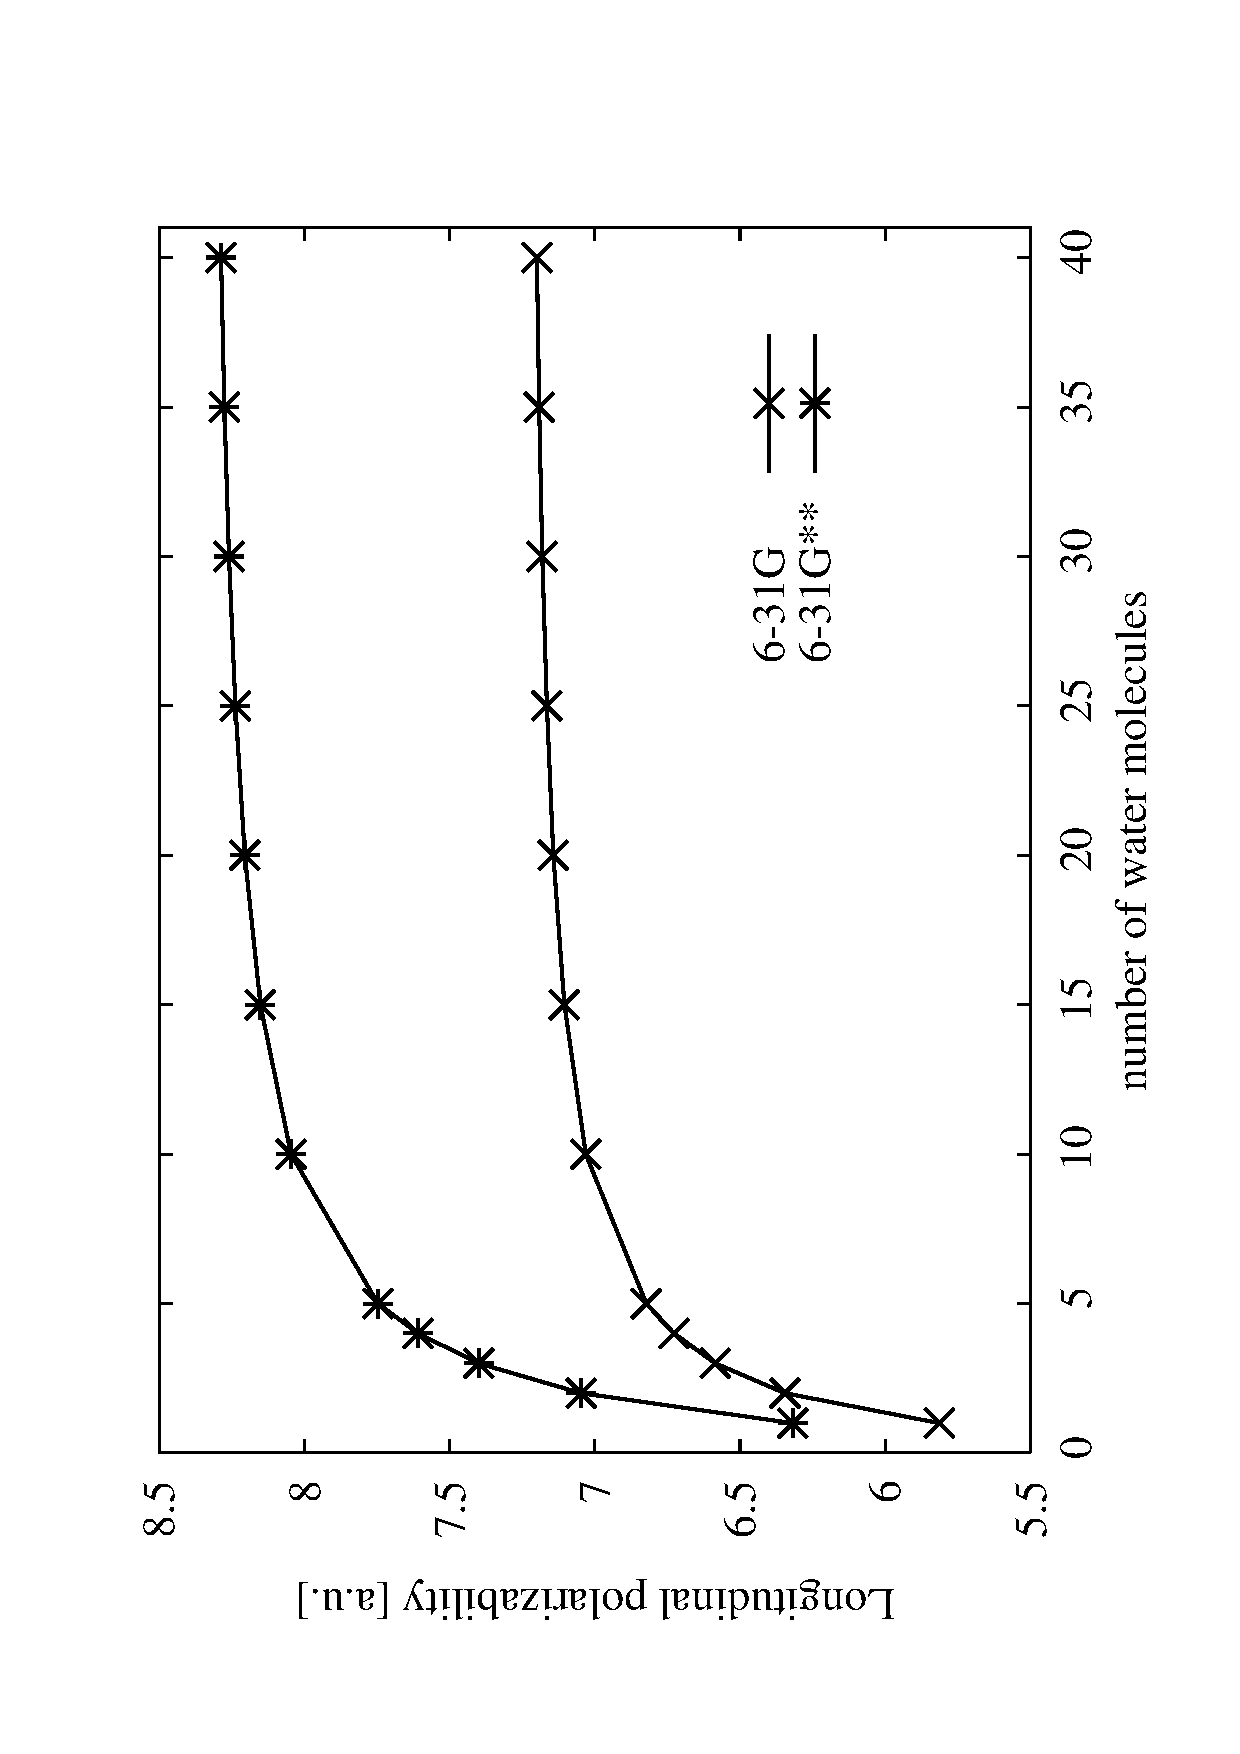
\includegraphics[angle=-90.00]{Alpha_All}}
\end{figure}


\begin{figure}[t]
  \caption{\protect
    Longitudinal first hyperpolarizability per water molecule for 
    the 6-31G and 6-31G** basis sets in function
    of the number of water molecule in the chain.
  }\label{fig:Beta_All}
  \resizebox*{3.5in}{!}{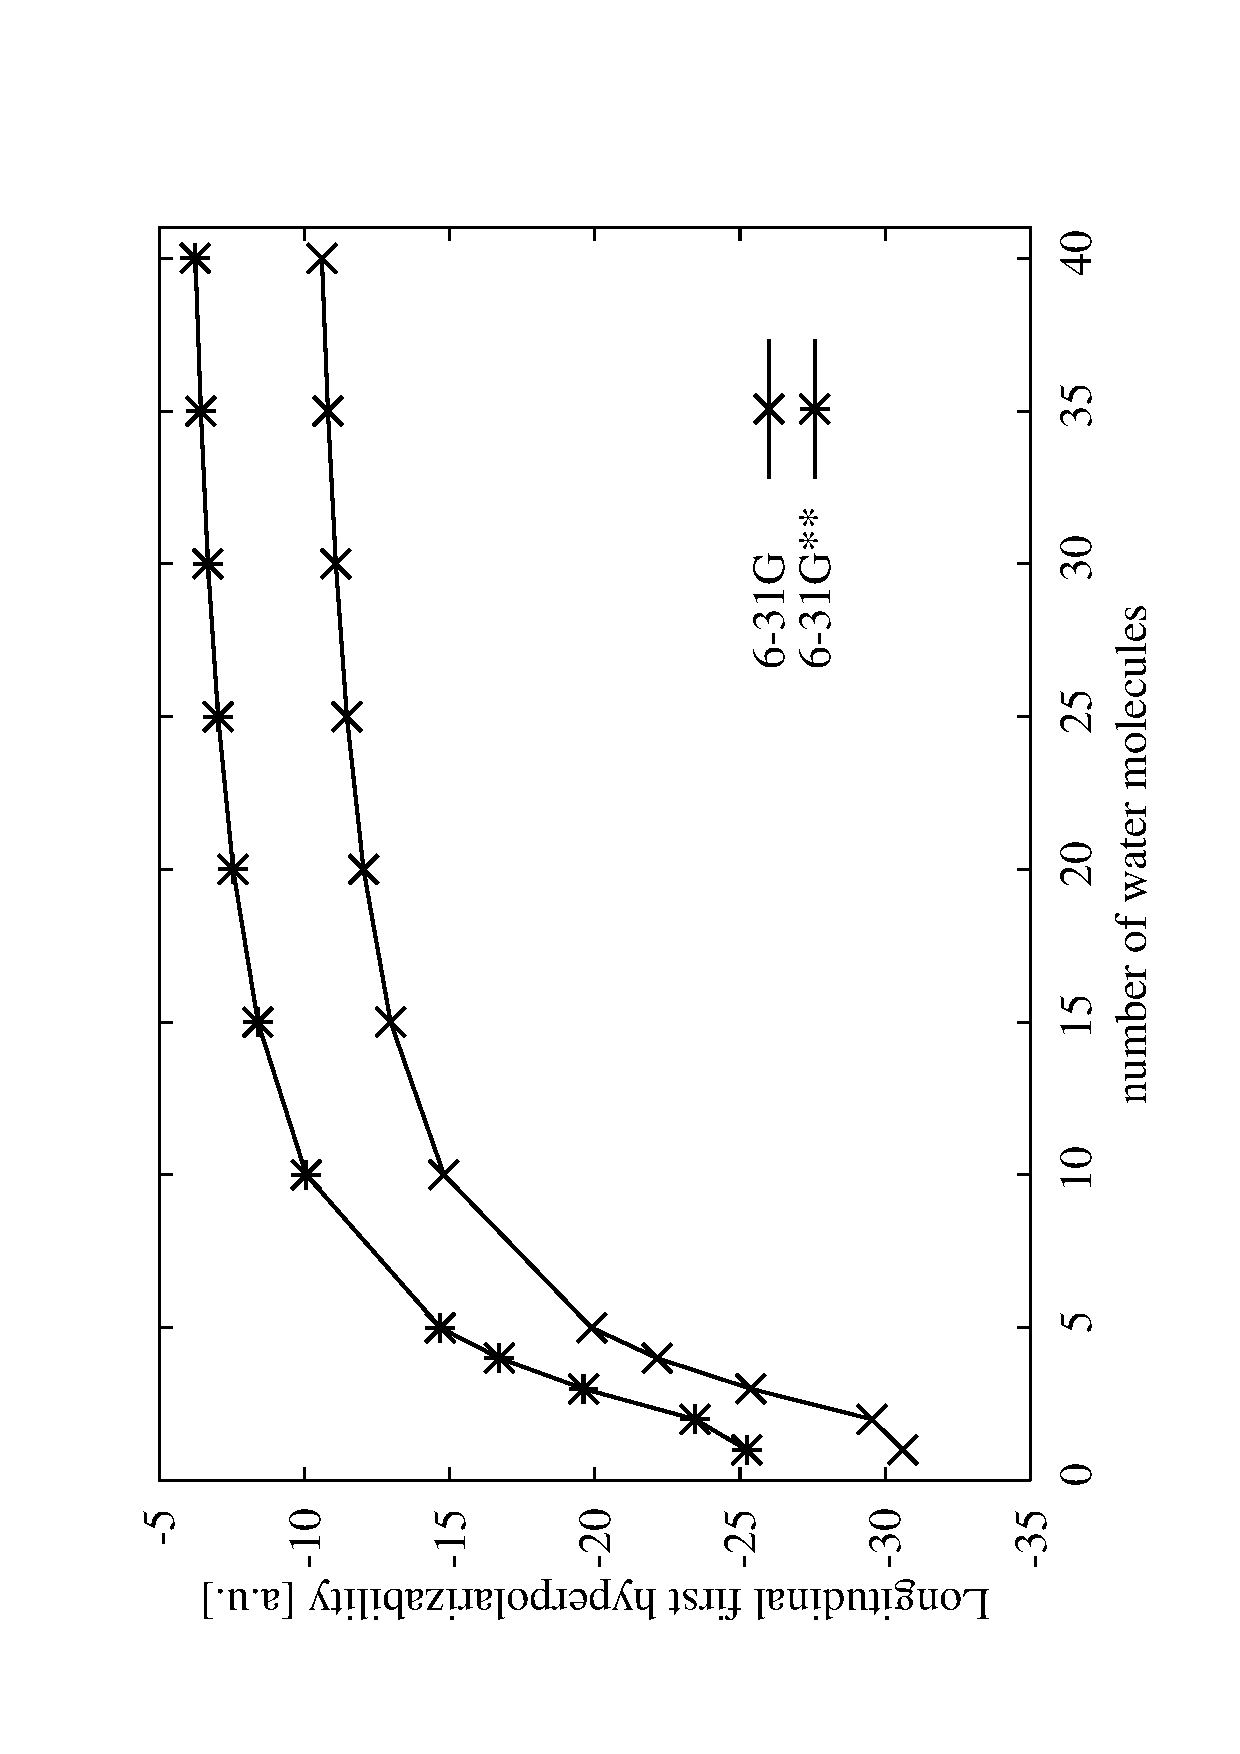
\includegraphics[angle=-90.00]{Beta_All}}
\end{figure}


\begin{figure}[t]
  \caption{\protect
    Longitudinal second hyperpolarizability per water molecule for 
    the 6-31G and 6-31G** basis sets in function
    of the number of water molecule in the chain.
  }\label{fig:Gamma_All}
  \resizebox*{3.5in}{!}{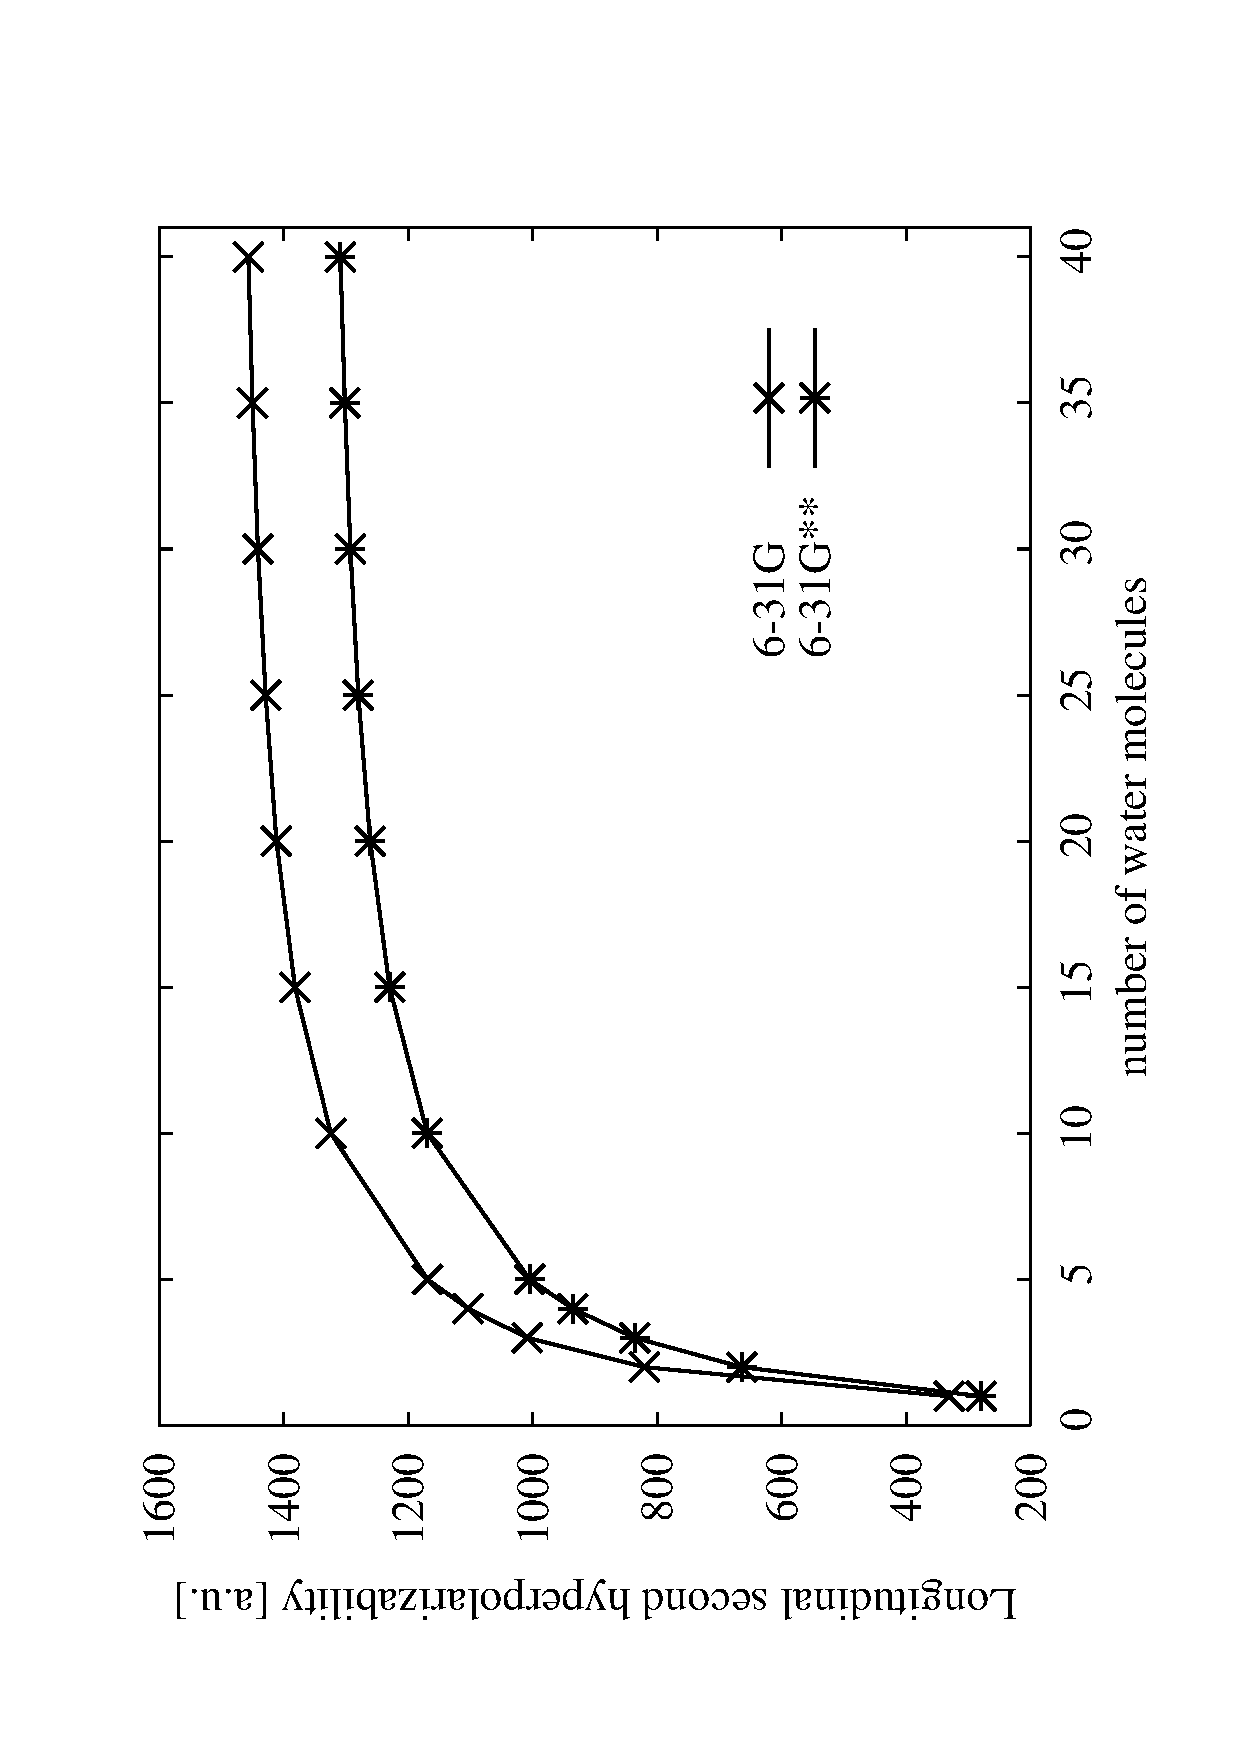
\includegraphics[angle=-90.00]{Gamma_All}}
\end{figure}


\begin{table}
  \centering
  \caption{\protect
    Longitudinal polarizability $\alpha_{zz}$
    for different water chain lengths with the 6-31G and 6-31G** basis sets
    and $Tight$ accuracy (See text) and the results obtained with
    the GAMESS quantum chemistry package \cite{gamess} with the 6-31G. 
    All the results are in $[a.u.]$.
  }\label{tab:Polari_1D_Values}
  \begin{ruledtabular}
    \begin{tabular}{cccc}
      $N$ &\multicolumn{1}{c}{6-31G\footnotemark[1]}
      &\multicolumn{1}{c}{6-31G\footnotemark[2]}
      &\multicolumn{1}{c}{6-31G**\footnotemark[2]}\\
      \hline
      1 & 5.8136 & 5.813589 & 6.318837     \\
      2 & 6.3448 & 6.344830 & 7.047412     \\
      3 & 6.5844 & 6.584449 & 7.399737     \\
      4 & 6.7276 & 6.727684 & 7.609261     \\
      5 & 6.8226 & 6.822640 & 7.746704     \\
     10 & 7.0308 & 7.030870 & 8.045561     \\
     15 & 7.1047 & 7.104780 & 8.151306     \\
     20 & 7.1424 & 7.142433 & 8.205162     \\
     25 & 7.1652 & 7.165231 & 8.237774     \\
     30 & 7.1805 & 7.180514 & 8.259633     \\
     35 & 7.1914 & 7.191468 & 8.275303     \\
     40 & 7.1996 & 7.199704 & 8.287090     \\
    \end{tabular}
  \end{ruledtabular}
 \footnotetext[1]{GAMESS calculations.}
 \footnotetext[2]{MondoSCF calculations.}
\end{table}

%# Grendels, serial
%#  h2o 1D,6-31G,6-31G**, Good,Tight, TC2, TC2R
%#            6-31G                 6-31G**
%##h2o   Good       Tight      Good       Tight  
%   1  5.816843   5.813589   6.318880   6.318837
%   2  6.347806   6.344830   7.047533   7.047412
%   3  6.586309   6.584449   7.401679   7.399737
%   4  6.737115   6.727684   7.609359   7.609261
%   5  6.822869   6.822640   7.746792   7.746704
%  10  7.031173   7.030870   8.045755   8.045561
%  15  7.105109   7.104780   8.151490   8.151306
%  20  7.142874   7.142433   8.205483   8.205162
%  25  7.165841   7.165231   8.238139   8.237774
%  30  7.180868   7.180514   8.260017   8.259633
%  35  7.191806   7.191468   8.275722   8.275303
%  40  7.200072   7.199704   8.287543   8.287090

%GAMESS GAMESS GAMESS GAMESS GAMESS GAMESS GAMESS GAMESS GAMESS 
%1     5.8136  5.8136   30.6125  30.6125    330.5753   330.5753
%2    12.6896  6.3448   59.0887  29.5444   1640.2796   820.1398
%3    19.7533  6.5844   76.1089  25.3696   3025.6968  1008.5656
%4    26.9106  6.7276   88.5646  22.1411   4413.9253  1103.4813
%5    34.1130  6.8226   99.4626  19.8925   5844.7817  1168.9563
%10   70.3083  7.0308  148.0633  14.8063  13242.9057  1324.2906
%15  106.5710  7.1047  194.5692  12.9713  20727.9867  1381.8657
%20  142.8477  7.1424  240.6673  12.0334  28228.5295  1411.4264
%25  179.1295  7.1652  286.6190  11.4648  35734.4198  1429.3767
%30  215.4138  7.1805  332.5018  11.0834  43242.7849  1441.4261
%35  251.6995  7.1914  378.3465  10.8099  50752.4976  1450.0713
%40  287.9861  7.1996  424.1681  10.6042  58263.0262  1456.5756
%GAMESS GAMESS GAMESS GAMESS GAMESS GAMESS GAMESS GAMESS GAMESS 


\begin{table}
  \centering
  \caption{\protect
    Longitudinal polarizability $\beta_{zzz}$
    for different water chain lengths with the 6-31G and 6-31G** basis sets
    and $Tight$ accuracy (See text) and the results obtained with
    the GAMESS quantum chemistry package \cite{gamess} with the 6-31G. 
    All the results are in $[a.u.]$.
  }\label{tab:Polari_1D_Values}
  \begin{ruledtabular}
    \begin{tabular}{ccccc}
      $N$ &\multicolumn{1}{c}{6-31G\footnotemark[1]}
      &\multicolumn{1}{c}{6-31G\footnotemark[2]}
      &\multicolumn{1}{c}{6-31G\footnotemark[2]\footnotemark[3]}
      &\multicolumn{1}{c}{6-31G**\footnotemark[2]}\\
      \hline
      1 & -30.6125 & -30.612178 & -30.612274 & -25.232854 \\
      2 & -29.5444 & -29.545096 & -29.545207 & -23.454776 \\
      3 & -25.3696 & -25.370516 & -25.370628 & -19.611398 \\
      4 & -22.1411 & -22.141553 & -22.141869 & -16.713840 \\
      5 & -19.8925 & -19.893306 & -19.893441 & -14.683861 \\
     10 & -14.8063 & -14.807203 & -14.807392 & -10.065481 \\
     15 & -12.9713 & -12.972171 & -12.972379 &  -8.396753 \\
     20 & -12.0334 & -12.034259 & -12.034505 &  -7.544200 \\
     25 & -11.4648 & -11.465624 & -11.465915 &  -7.027523 \\
     30 & -11.0834 & -11.084234 & -11.084569 &  -6.680997 \\
     35 & -10.8099 & -10.810645 & -10.811061 &  -6.432514 \\
     40 & -10.6042 & -10.604860 & -10.605360 &  -6.245644 \\
    \end{tabular}
  \end{ruledtabular}
 \footnotetext[1]{GAMESS calculations.}
 \footnotetext[2]{MondoSCF calculations.}
 \footnotetext[3]{The density matrix based 2n+1 rule has been used.}
\end{table}

%# Grendels, serial
%#  h2o 1D,6-31G,6-31G**, Good,Tight, TC2, TC2R
%#             6-31G                 6-31G**
%##h2o    Good       Tight      Good       Tight  
%   1 -30.608433 -30.612178 -25.232553 -25.232854
%   2 -29.545590 -29.545096 -23.455425 -23.454776
%   3 -25.371724 -25.370516 -19.610785 -19.611398
%   4 -22.139294 -22.141553 -16.713768 -16.713840
%   5 -19.895058 -19.893306 -14.686577 -14.683861
%  10 -14.807930 -14.807203 -10.078511 -10.065481
%  15 -12.970406 -12.972171  -8.408976  -8.396753
%  20 -12.030914 -12.034259  -7.559121  -7.544200
%  25 -11.457680 -11.465624  -7.030470  -7.027523
%  30 -11.067331 -11.084234  -6.691950  -6.680997
%  35 -10.825402 -10.810645  -6.442292  -6.432514
%  40 -10.507809 -10.604860  -6.250695  -6.245644



\begin{table}
  \centering
  \caption{\protect
    Longitudinal polarizability $\gamma_{zzzz}$
    for different water chain lengths with the 6-31G and 6-31G** basis sets
    and $Tight$ accuracy (See text) and the results obtained with
    the GAMESS quantum chemistry package \cite{gamess} with the 6-31G. 
    All the results are in $[a.u.]$.
  }\label{tab:Polari_1D_Values}
  \begin{ruledtabular}
    \begin{tabular}{cccc}
      $N$ &\multicolumn{1}{c}{6-31G\footnotemark[1]}
      &\multicolumn{1}{c}{6-31G\footnotemark[2]}
      &\multicolumn{1}{c}{6-31G**\footnotemark[2]}\\
      \hline
      1 &  330.5753 &  330.577009 &  278.898509 \\
      2 &  820.1398 &  820.160650 &  663.493200 \\
      3 & 1008.5656 & 1008.580733 &  836.073966 \\
      4 & 1103.4813 & 1103.494950 &  935.378474 \\
      5 & 1168.9563 & 1168.972479 & 1004.896120 \\
     10 & 1324.2906 & 1324.304700 & 1169.020999 \\
     15 & 1381.8657 & 1381.882600 & 1229.747000 \\
     20 & 1411.4264 & 1411.448699 & 1260.928449 \\
     25 & 1429.3767 & 1428.980999 & 1279.877079 \\
     30 & 1441.4261 & 1441.474333 & 1292.603933 \\
     35 & 1450.0713 & 1450.143685 & 1301.746485 \\
     40 & 1456.5756 & 1456.682800 & 1308.644675 \\
    \end{tabular}
  \end{ruledtabular}
 \footnotetext[1]{GAMESS calculations.}
 \footnotetext[2]{MondoSCF calculations.}
\end{table}

%# Grendels, serial
%#  h2o 1D,6-31G,6-31G**, Good,Tight, TC2, TC2R
%#               6-31G                     6-31G**
%##h2o     Good         Tight        Good       Tight  
%   1   330.500720   330.577009   278.906999   278.898509
%   2   820.172599   820.160650   663.493749   663.493200
%   3  1008.563066  1008.580733   836.049133   836.073966
%   4  1103.520725  1103.494950   935.288549   935.378474
%   5  1169.048159  1168.972479  1005.069079  1004.896120
%  10  1325.171700  1324.304700  1169.970399  1169.020999
%  15  1383.163933  1381.882600  1230.688333  1229.747000
%  20  1414.483850  1411.448699  1261.845550  1260.928449
%  25  1435.599519  1428.980999  1280.417440  1279.877079
%  30  1452.626633  1441.474333  1293.059166  1292.603933
%  35  1468.606228  1450.143685  1301.725400  1301.746485
%  40  1484.647500  1456.682800  1308.446325  1308.644675


\subsection{Linear scaling: 3D water clusters}
3D water clusters show an early onset of linear scaling for accrurate
basis set and low tresholds and higher order response.

The density responses matrices show an exponential decay as a function
of the internuclear distance, however the decay is slower and the locality
becomes lower for the higher order response functions.
Therefor, we find a later onset for the linear scaling for the higher order
responses.



\begin{figure}[t]
  \caption{\protect
    Total WALL time of the fifth first order CPSCF iteration for
    the water cluster sequence with the 6-31G and 6-31G** 
    basis sets and the {\tt GOOD} and {\tt TIGHT} 
    numerical thresholds (see text) controlling numerical
    precision of the result. The lines are fits to the 
    last three and four points, respectively.
  }\label{Alpha_scaling}
  \resizebox*{3.5in}{!}{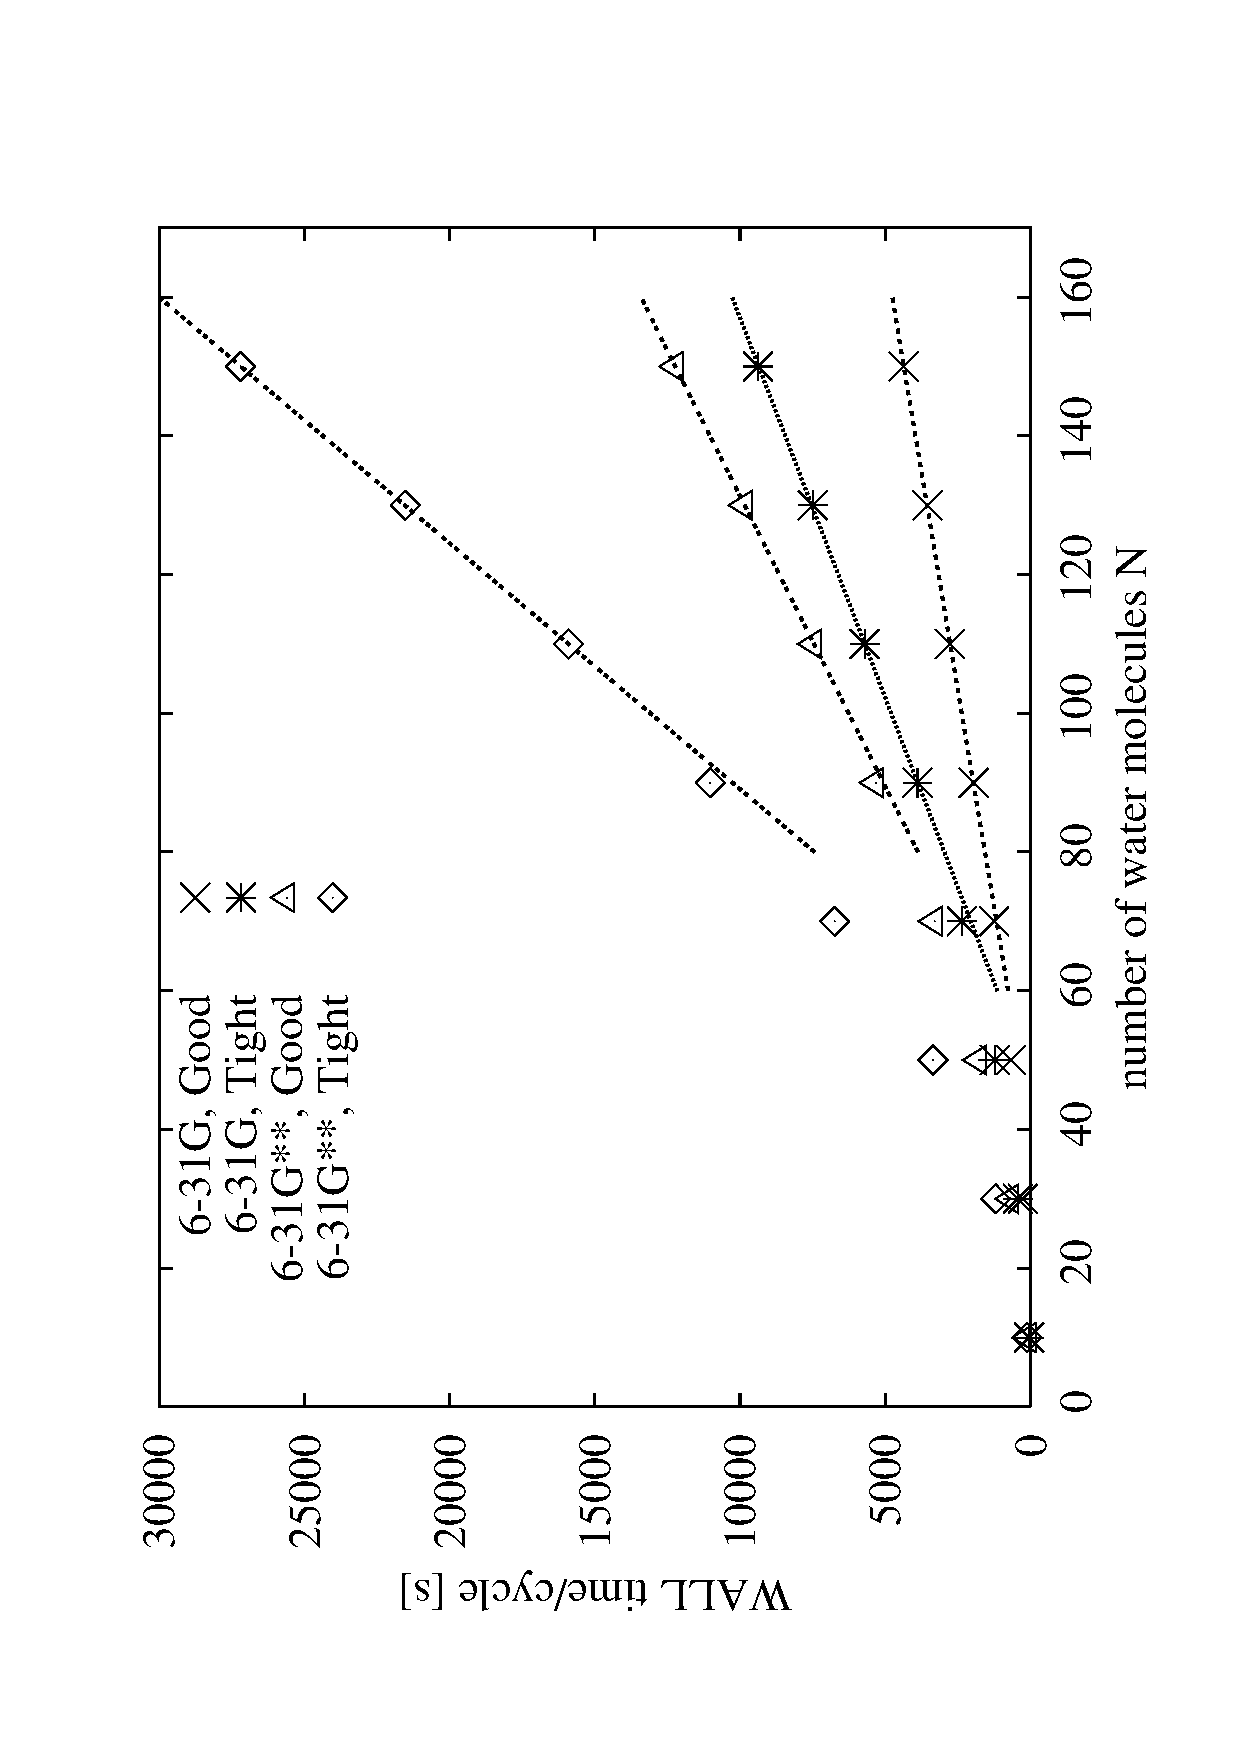
\includegraphics[angle=-90.00]
                        {Alpha_h2o3D_6-31G_6-31Gss_G_T_t}}
\end{figure}


\begin{figure}[t]
  \caption{\protect
    Total WALL time of the fifth second order CPSCF iteration for
    the water cluster sequence with the 6-31G and 6-31G** 
    basis sets and the {\tt GOOD} and {\tt TIGHT} 
    numerical thresholds (see text) controlling numerical
    precision of the result. The lines are fits to the 
    last three and four points, respectively.
  }\label{Beta_scaling}
  \resizebox*{3.5in}{!}{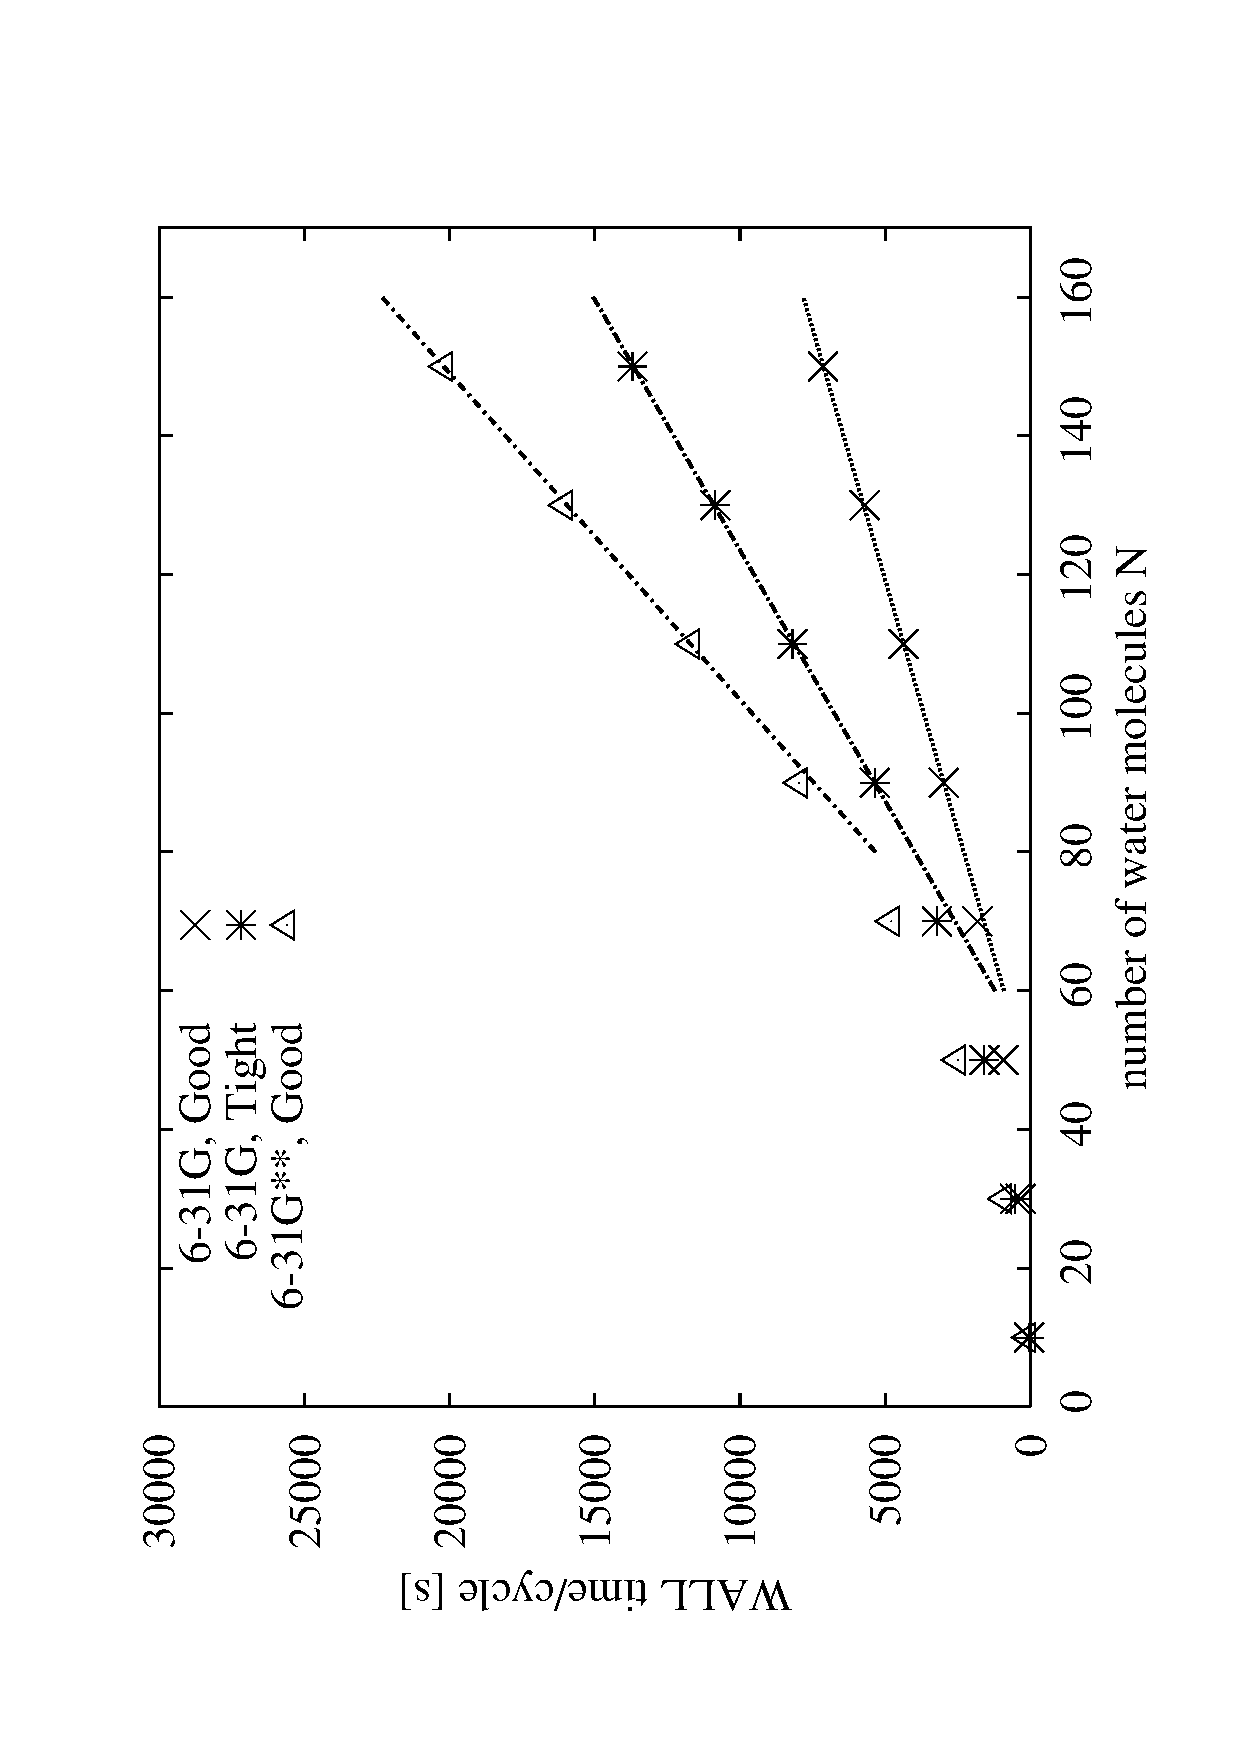
\includegraphics[angle=-90.00]
                        {Beta_h2o3D_6-31G_6-31Gss_G_T_t}}
\end{figure}


\begin{figure}[t]
  \caption{\protect
    Total WALL time of the fifth third order CPSCF iteration for
    the water cluster sequence with the 6-31G and 6-31G** 
    basis sets and the {\tt GOOD} and {\tt TIGHT} 
    numerical thresholds (see text) controlling numerical
    precision of the result. The lines are fits to the 
    last three and four points, respectively.
  }\label{Beta_scaling}
  \resizebox*{3.5in}{!}{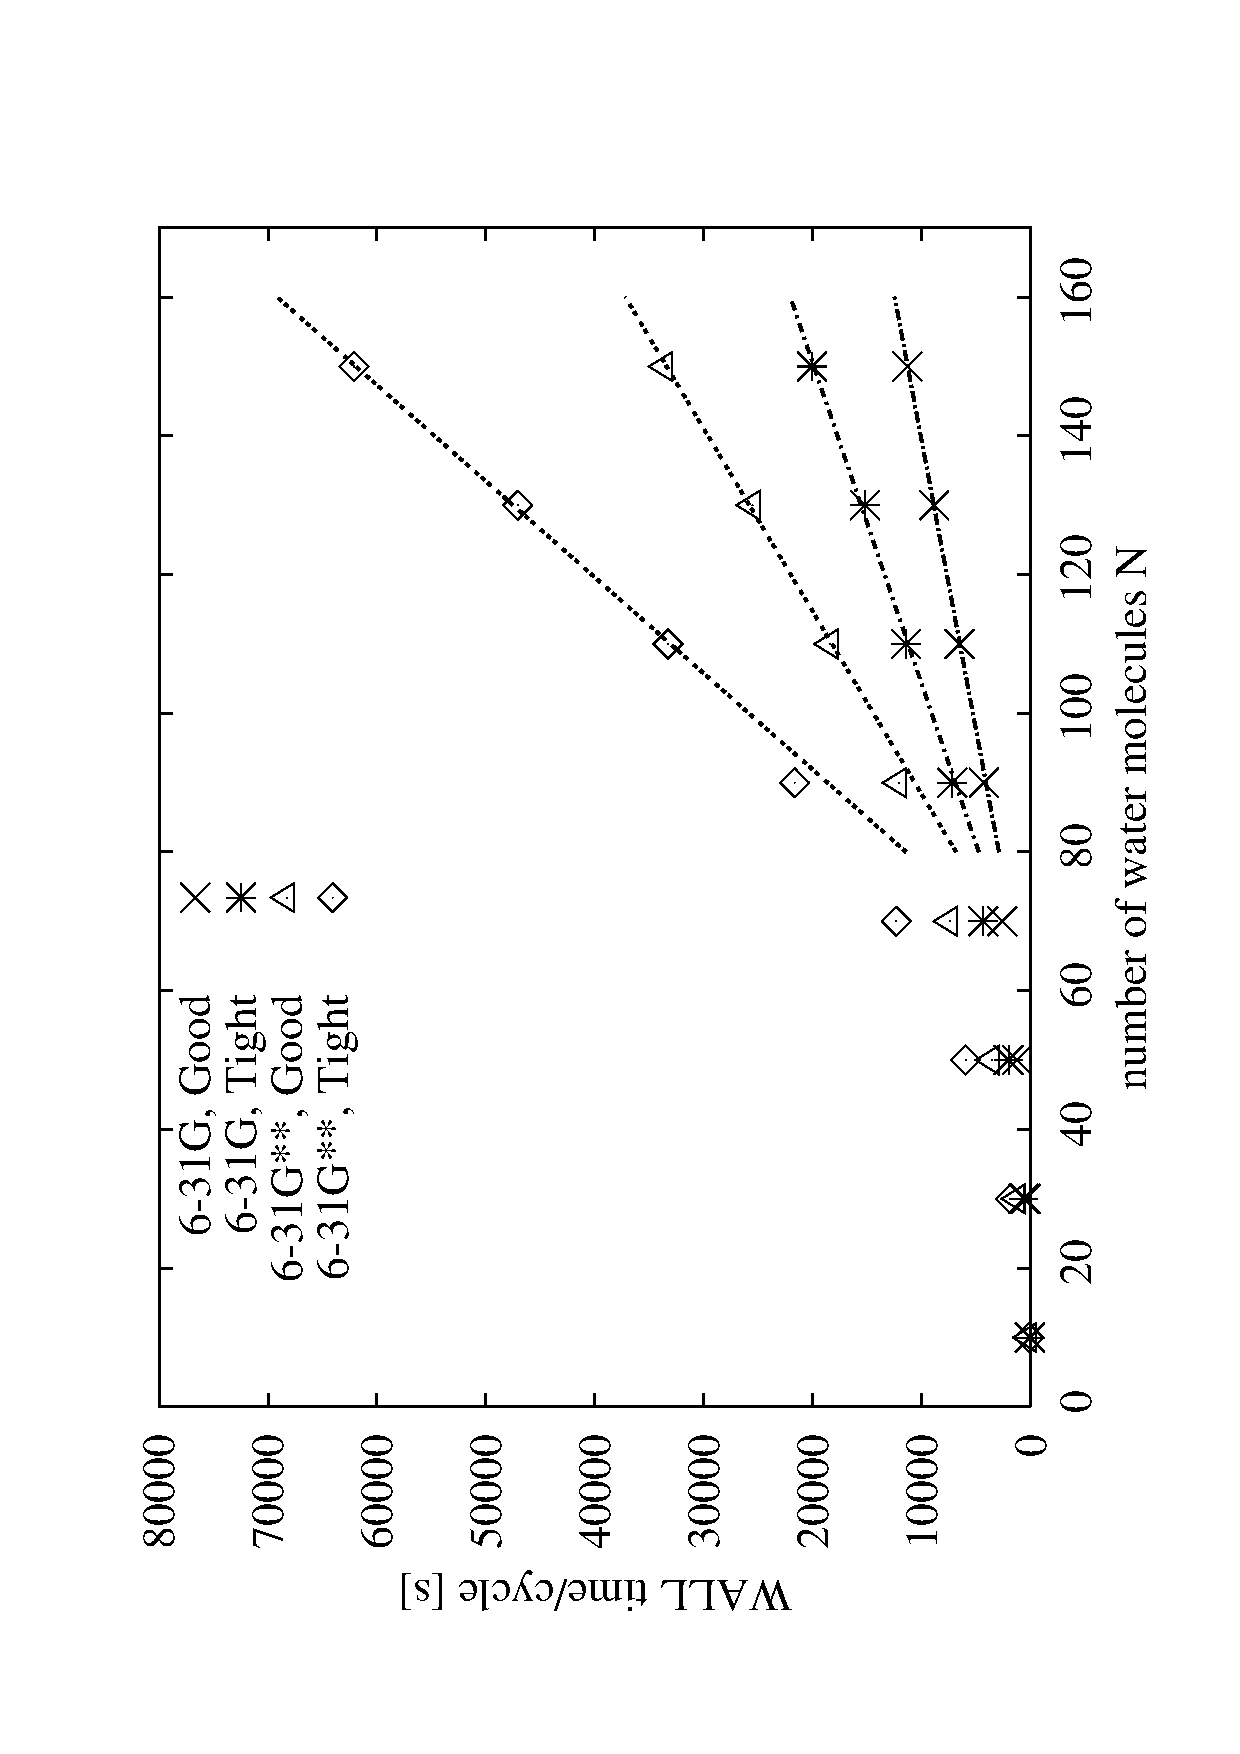
\includegraphics[angle=-90.00]
                        {Gamma_h2o3D_6-31G_6-31Gss_G_T_t}}
\end{figure}



\begin{figure}[t]
  \caption{\protect
    Total WALL time of the fifth first, second and third order
    CPSCF iteration for the water cluster sequence with the 6-31G
    basis set and the {\tt GOOD} numerical threshold (see text) 
    controlling numerical precision of the result. The lines
    are fits to the last three and four points, respectively.
  }\label{Alpha_scaling}
  \resizebox*{3.5in}{!}{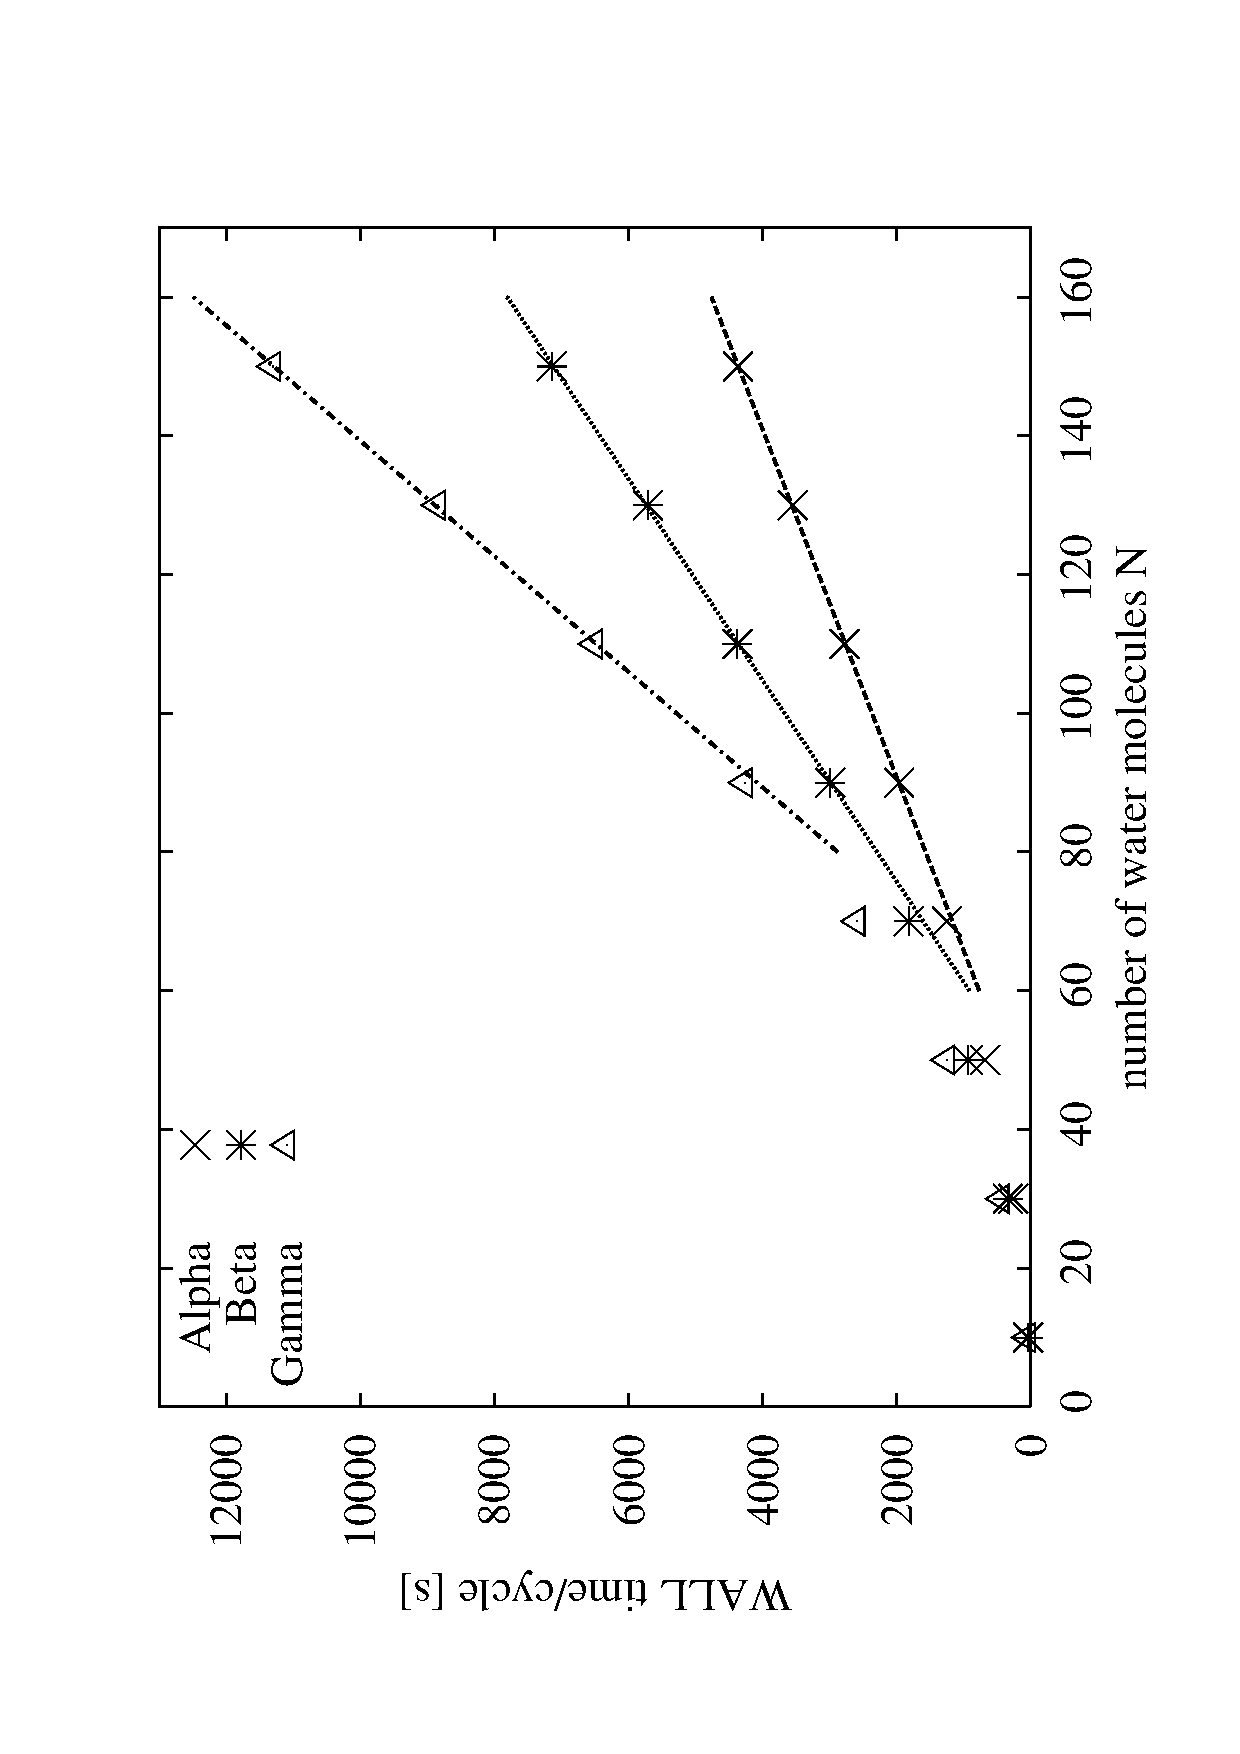
\includegraphics[angle=-90.00]
                        {Mix_h2o3D_6-31G_6-31Gss_G_T_t}}
\end{figure}



%\subsubsection{}
\subsection{Exponential decay}


\begin{figure}[t]
  \caption{\protect
    Magnitudes of the RHF/6-31G density matrix derivative elements 
    along the z axis with the separation of basis function centers
    for the $(H_2O)_{150}$ water cluster. The density matrix 
    derivative has been converged to within Tight (e.g. 
    matrix threshold of $10^{-6}$ $[a.u.]$).
  }\label{fig:Alpha_Decay}
%  \resizebox*{3.5in}{!}{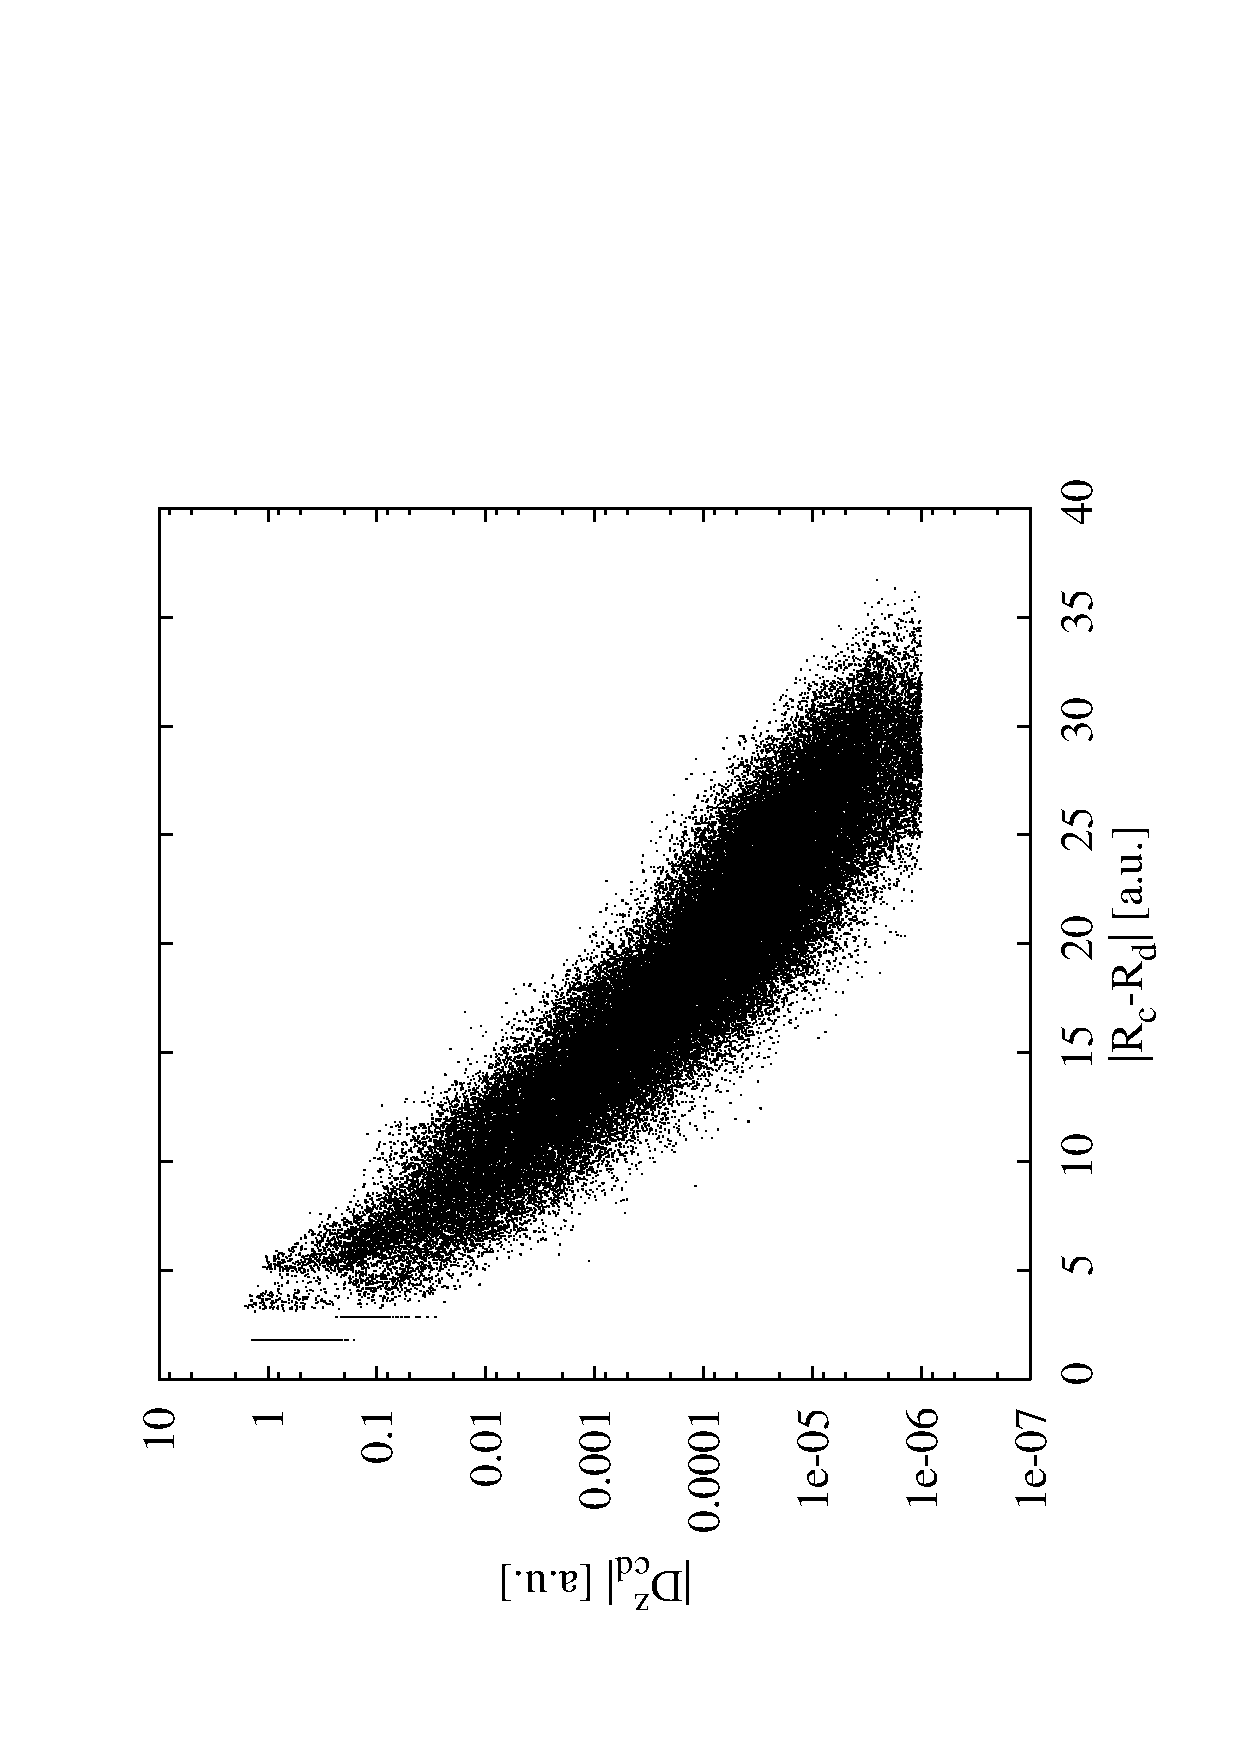
\includegraphics[angle=-90.00]{Alpha_Decay_Z_6-31G}}
\end{figure}


%\section{}
%\subsection{Discusion}




%%%%%%%%%%%%%%%%%%%%%%%%%%%%%%%%%%%%%%%%%%%%%%%%%%%%%%%%%%%%%%%%
%%%%%%%%%%%%%%%%%%%%%%%%%%%%%%%%%%%%%%%%%%%%%%%%%%%%%%%%%%%%%%%%
\section{Sumary and Conclusion}


 We have proposed and demonstreted a linear scaling self
 consisitent sheme for high order response peoperties.
 The sheme solves the coupled perturbed self consitent field 
 equation by the perturbed projection method.


% It is applied to the computation
% of the first and second electric hyperpolarizabilities of three
% dimensional water clusters. Linear scaling and locality of the response
% densities are demonstrated. 

%%%%%%%%%%%%%%%%%%%%%%%%%%%%%%%%%%%%%%%%%%%%%%%%%%%%%%%%%%%%%%%%
%%%%%%%%%%%%%%%%%%%%%%%%%%%%%%%%%%%%%%%%%%%%%%%%%%%%%%%%%%%%%%%%
%Acknowledgements
\begin{acknowledgments}
 This work has been supported by the US Department of Energy 
 under contract ???????????? and the ASCI project.  
 The Advanced Computing Laboratory of Los 
 Alamos National Laboratory is acknowledged.
 All the numerical computations have been
 performed on computing resources located at this facility.
\end{acknowledgments}
%%%%%%%%%%%%%%%%%%%%%%%%%%%%%%%%%%%%%%%%%%%%%%%%%%%%%%%%%%%%%%%%
%%%%%%%%%%%%%%%%%%%%%%%%%%%%%%%%%%%%%%%%%%%%%%%%%%%%%%%%%%%%%%%%
\bibliography{Response3}
%%%%%%%%%%%%%%%%%%%%%%%%%%%%%%%%%%%%%%%%%%%%%%%%%%%%%%%%%%%%%%%%
%%%%%%%%%%%%%%%%%%%%%%%%%%%%%%%%%%%%%%%%%%%%%%%%%%%%%%%%%%%%%%%%
%%%%%%%%%%%%%%%%%%%%%%%%%%%%%%%%%%%%%%%%%%%%%%%%%%%%%%%%%%%%%%%%
%%%%%%%%%%%%%%%%%%%%%%%%%%%%%%%%%%%%%%%%%%%%%%%%%%%%%%%%%%%%%%%%
%%%%%%%%%%%%%%%%%%%%%%%%%%%%%%%%%%%%%%%%%%%%%%%%%%%%%%%%%%%%%%%%
\end{document}
%
% ****** End of file apssamp.tex ******
